The chip apparatus was assembled for preliminary tests, but isolated from the 
main \CaF{} experiment. This modest setup was useful for a variety of
measurements, which will be discussed below, including vacuum compatibility,
current testing under vacuum, and looking at the amount of background scatter
from the apparatus during imaging. We anticipate background scatter to be a
significant challenge in an experiment close to a surface, and discuss
possibilities for a background-free imaging scheme in
section~\ref{exper:bgf}.

\section{Experiment assembly}

In this section we will give details of the apparatus, especially the chip
flange assembly, which was introduced at the end of chapter~\ref{overview}. The
flange assembly is designed to hold the chip in position for loading \CaF{},
whilst also providing current delivery and heat sinking. Considerations have
been made for future experiments using microwaves, with two high-frequency
microwave feedthroughs incorporated as well. The flange was manufactured by
Allectra GmbH, and the heat sink was machined in the Imperial College workshop.
A detailed view is shown in \myfigref{overview:fig:chipchamber}.

The copper heat sink is mounted to the flange using screws where the thread has
been partially removed. This is done to precent any trapped gas causing virtual
leaks inside the chamber. The heat sink supports the subchip and also
incorporates the large U-trap, which is recessed beneath the chip. It is
electrically isolated from the heat sink by \AlN{} plates. This material is
chosen since it is an electrical insulator, but will still allow the conduction
of heat away from the U-wire whilst being UHV compatible. The subchip is
attached to the heat sink with metal screws. Since the conductor tracks are at
points very close to the mounting holes, we isolate the screws from the surface
using washers made from polyimide (another UHV compatible insulator) which were
manufactured in the College workshop.

The current is delivered to the U-wire through two high-current feedthroughs.
For the chip currents, the 16-pin feedthrough is used, and is connected to the
subchip by kapton-coated wires from LewVac. When connecting the wires to the
subchip we use polyimide bushings (also made in the College workshop) to ensure
that they are electrically isolated from the aluminium core of the PCB.

The flange is mounted in the chip chamber, a DN63 cube chamber from Kurt J.
Lesker Co.\ (KJL) whose configuration is shown in \myfigref{exper:fig:exper}.
The assembly is designed so that molecules will enter the chamber along an axis
that is \SI{3}{\milli\meter} from the surface of the chip. A tee is installed
to allow for additional vacuum ports whilst still allowing a clear line of
sight across the chip surface. This is shown in the figure by the pink arrow,
and passes through twhothrough the viewports AR-coated viewports, also from
KJL, as shown in the figure. This provides optical access across the surface of
the chip for illumination.  Onto the tee we attach a \cm{turbo pump}, backed by
a scroll (not pictured).  There is also a DN63-DN40 adapter opposite the chip
flange, this will be where the chamber is attached to the \CaF{} experiment in
the future, but for testing purposes a \cm{pirani gauge or RGA} is attached
instead.

\begin{figure}
  \centering
  \includegraphics[width=\textwidth]{figs/exper/exper.pdf}
  \caption{A top-down (a) and profile (b) view of the chip experiment. In (a)
  we show the line of sight through the chamber by the pink arrow. In (b) we
  show a view as if looking through the viewport on the tee, and also highlight
  the position of the interior lens inside the chamber. Here the
  pink arrow denotes the path of light collected for imaging from beneath the
  chip.}
  \label{exper:fig:exper}
\end{figure}

The optical access allows for two main styles of imaging experiment. In both, a
laser beam will enter through the viewports as shown in
\mysubfigref{exper:fig:exper}{a}. Light-induced fluorescence can then be imaged
by collecting the light along this axis, this would allow measurement of the
changing height of molecules that are released from the trap as they fall under
gravity. 
%
An alternative arrangement is shown in in \mysubfigref{exper:fig:exper}{b},
where light is collected from a viewport beneath the chip and imaged onto a
CCD. This may be useful since it avoids imaging along the path of the light
driving the transitions and could reduce background scatter. We anticipate
background scatter to be a significant problem for an experiment that is
conducted close to what essentially amounts to a giant mirror, and this scheme
will be discussed further in section~\ref{exper:scatter}.

Finally, we note that the current drivers for the experiment were not completed
as part of this project. Instead, a simple regulated power supply and
field-effect transistor (FET) switch were used to control current pulses for
testing. This will be discussed in section~\ref{exper:current}.

\section{Vacuum testing}

For testing the vacuum compatability of the experiment, the RGA is attached to
the chamber. To reach UHV pressures, it is required to bake the experiment.
Heater tape is applied and the chamber is wrapped in foil, the temperature is
then raised over the course of a \cm{few hours} to \cm{over 100 degrees.}  It
is held at this temperature for \cm{atleast 48 hours}, before being ramped back
down. This removes excess water vapour from inside the chamber, and expells any
water that has been absorbed into the chamber walls.

The chamber was first leak checked~\cite{} and then brought to UHV pressure
with the chip flange assembly replaced with a blank. This provided a baseline
pressure for the chamber. We then swapped in the flange assembly, and repeated
the bakeout process with various iterations of our design. In our design
process we were careful to choose materials that are UHV compatible but it was
important to check that the assembly could reach the pressures required. In
particular we were concerned with the Epoxy Technology glue, since any errors
in the mixing and application procedure could cause outgassing, and the solder,
which was not rated for UHV uses.

To measure the pressure of the chamber an RGA scan is undertaken, with the
resulting partial pressures shown with and without the chip assembly in
\myfigref{exper:fig:rga}. The total pressure (the sum of the partial pressures)
is \SI{5.0E-10}{\milli\bar} and \SI{8.8E-10}{\milli\bar} in each case respectively. The scan with the chip assembly
has a similar shape to the empty chamber scan, but with slightly higher values.
In both, we see the typical peaks for hydrogen (2), water (18) and nitrogen
(28), which dominate the spectrum. This is typical of a scan through a UHV
system~\cite{}, and suggests that the chip assembly does not introduce any
sources of contamination or outgassing into the experiment.
%
Further tests were conducted when using a chip with wirebonds rather than
solder, and the microwave barell connectors and launchers (see
section~\ref{mws:integrating}) which will be required for future experiments.
These yielded similar results to those discussed above, with no discernable
change in the pressure.

  \begin{figure}[htb]
  \centering
  \begin{tikzpicture}
    \begin{axis}[
        ymode=log,
        enlargelimits=true,
        xlabel=Mass number,
        ylabel=Partial pressure (\si{\milli\bar}),
        width=0.8\textwidth,
        height = 0.4\textwidth,
        legend pos=north east,
        x tick label style={/pgf/number format/.cd, set thousands separator={}},
        ylabel style={yshift=10pt}
    ]
      \addplot [thick, color=blue] table {figs/exper/rga/emptyData.dat};
      \addlegendentry{Empty chamber};
      \addplot [thick, color=pink] table {figs/exper/rga/chipData.dat};
      \addlegendentry{Chip assembly};
    \end{axis}
  \end{tikzpicture}
  \caption{RGA scan for the chip chamber assembly when empty, and when loaded
  with the chip flange assembly.}
  \label{exper:fig:rga}
\end{figure}


\section{Current testing}
\label{exper:current}
% TODO I think maybe this should go above vacuum tests?

It was also important to test the currents that can be achieved through the
chip trapping wires. These tests were conducted with the chip under vacuum
($P<10^{-6}\si{\milli\bar}$) and using the setup shown in
\myfigref{exper:fig:curtest}, which was used since our custom current drivers
where not ready at this stage. A regulated power supply delivers a current to
the chip, controlled by the FET circuit that is in turn switched by a signal
generator. This gives us control over the pulse length, and allows us to
deliver voltage $V_\text{PSU}$ up to \SI{30}{\volt} to the chip, represnted
here by the resistor $R_\text{load}$. The current through the chip can be
measured via the potential difference across $R_\text{sense} = \SI{0.5}{\ohm}$.

% TODO Do Acknowledge symbols with cite
% https://commons.wikimedia.org/wiki/File:Electrical_symbols_library.svg
\begin{figure}[htb]
  \centering
  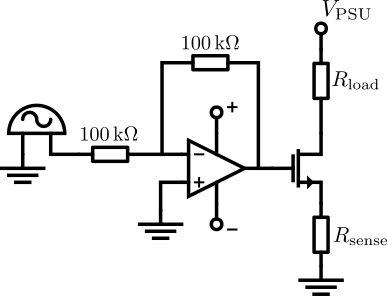
\includegraphics[width=0.5\textwidth]{figs/exper/circuit.pdf}
  \caption{The electronic circuit used to test the chip wires. The chip is
  represented by resistor $R_\text{load}$. The operational amplifier is powered
  by a separate power supply. This figure was produced using the elements in
the electrical symbols library~\cite{}.}
  \label{exper:fig:curtest}
\end{figure}

\subsection{Wirebond tests}

We originally tested a number of designs where the chip was connected to the
subchip with wirebonds using the method described in \cm{ref wirebond
subsection}. In these cases it was found that the wirebonds were unreliable at
high currents. It was possible to achieve pulses of several amperes through
even the small wires, but these were not reliably repeatable, and often
resulted in the wirebonds being broken.

These tests were conducted using a \SI{200}{\milli\second} pulse of current,
repeating every \SI{10}{\second}. The supply voltage was ramped up gradually,
and the current through the chip was measured via the potential difference
across the FET controller's sense resistor (see \myfigref{exper:fig:curtest}).
Several iterations of chips (with varying wire heights) were tested, using all
trapping wires. However no meaningful results for maximum attainable current
were found, as invariably the wirebonds would fail. This was eastablished by a
visual inspection of the chip, and checking the electrical continuity across
the trapping wires, and from the subchip to the chip.

We attempted to improve the maximum current by increasing the number of
wirebonds on each pad, and by improving the quality of the wirebond joints. We
found that the former yielded an improvement to the maximum current capacity,
but the quality of the wirebond joints was difficult to quantify. As a rule of
thumb, the wirebonds were re-done if they could not withstand a light tug from
a pair of tweezers. Ultimately the number of wirebonds that it was possible to
produce was limited by the width of the wirebond pad, and the width of the
wirebonder head. We could achieve approximately ten wirebonds per pad somewhat
reliably.

There are various options that could be used to increase the maximum current of
the wirebonds.  We considered using a ribon wirebond~\cite{}, which promises
higher current throughput by using a ribon-shaped wire rather than a round one.
This was not possible due to the unavailabliity of the the hardware at LCN.
Another option was to use higher-diameter wire, but instead we attempted to
directly solder the chip, as described in the next section.

\subsection{Solder tests}

An alternative to wirebonding is to directly solder the chip to the subchip.
This must be done carefully, as described in section~\ref{fab:solder} but
if done correctly it yields a highly stable electrical connection. \cm{The
UHV compatability of this method is discussed in a section to come (if I swap
the order around, which one?)} The same current tests were performed as for the 
wirebonded chips, as shown in \cm{the same fig or different?}. For solder
joints, the results were reliably repeatable, and we were able to observe
sufficient current densities for trapping (compared to those laid out in
section~\ref{overview:design}).

We consider a typical example of testing using the small wire
(\SI{9}{\micro\meter}), on a chip where the wire height achieved was
\SI{9}{\micro\meter}. Again, the current was pulsed on for
\SI{200}{\milli\second} once every \SI{10}{\second}, which we imagine to be
representative of a typical experiment. We show the current through the chip as
a function of supply density in \mysubfigref{exper:fig:current}{a}. Also shown
is a linear fit to the first ten data points. We observe here that for low
voltages, the current obeys Ohm's law, as we would expect, but this diverges
for higher voltages, suggesting that heating occurs in the device.

% Data from 2022-04-06_thesis_currenttest.nb (and from there just OneNote)
\begin{figure}[htb]
  \centering
  \begin{subfigure}[b]{0.45\textwidth}
  \begin{tikzpicture}
    \begin{axis}[
        enlargelimits=true,
        xlabel=$V$ (volts),
        ylabel=$I$ (amperes),
        width=\textwidth,
        height = \textwidth,
        x tick label style={/pgf/number format/.cd, set thousands separator={}},
        ylabel style={yshift=-8pt}
    ]
        \addplot [thick, blue, only marks] coordinates { (0.5, 0.1)(1, 0.28)(1.5, 0.46)(2, 0.64)(3, 1.04)(3.5, 1.2)(4, 1.4)(5, 1.7)(6, 2.2)(7, 2.6)(8, 2.8)(9, 3.)(10, 3.4)(11, 3.6)(12, 4.)(13, 4.4)(14, 4.6)(15, 4.8)(16, 5.)(17, 5.4)(18, 5.6)(19, 6.)(20, 6.)(21, 6.4)(22, 6.6)(23, 6.6)(24, 6.8) };
        \addplot[thick, pink, mark=none] coordinates {(0,-0.1136) (24,9.025)};
        \node[] at (axis cs: 1,8.5) {(a)};
      \end{axis}
  \end{tikzpicture}
  \end{subfigure}
  %
  \begin{subfigure}[b]{0.45\textwidth}
  \begin{tikzpicture}
    \begin{axis}[
        enlargelimits=true,
        xlabel=$I$ (amperes),
        ylabel=$R$ (ohm),
        width=\textwidth,
        height = \textwidth,
        x tick label style={/pgf/number format/.cd, set thousands separator={}},
        ylabel style={yshift=-8pt}
    ]
        \addplot [thick, blue, only marks] coordinates {
            (0.1, 2.7138)(0.28, 2.71005)(0.46, 2.70983)(0.64,
  2.71315)(1.04, 2.7332)(1.2, 2.74611)(1.4, 2.76617)(1.7,
  2.80446)(2.2, 2.89012)(2.6, 2.97829)(2.8, 3.02893)(3.,
  3.08393)(3.4, 3.20705)(3.6, 3.27515)(4., 3.42447)(4.4,
  3.59126)(4.6, 3.6812)(4.8, 3.77551)(5., 3.87419)(5.4,
  4.08465)(5.6, 4.19643)(6., 4.43309)(6., 4.43309)(6.4,
  4.68722)(6.6, 4.82084)(6.6, 4.82084)(6.8, 4.95882)
};
        \node[] at (axis cs: 1,8.5) {(b)};
      \end{axis}
  \end{tikzpicture}
  \end{subfigure}
  \caption{Increasing current in the small chip wire. The current is shown as a
  function of supply voltage in (a). The pink line shows a linear fit to the
  first ten points. In (b) this is converted into a resistance (as described in
the main text), which increases for higher currents.}
  \label{exper:fig:current}
\end{figure}

Nonetheless, with sufficient voltage it is possible to achieve currents of
\SI{6.8}{\ampere}, which  corresponds to a current density of
$j=\SI{6.8}{\ampere}/(\SI{9}{\micro\meter}\times\SI{9}{\micro\meter})=
\SI{8.4E10}{\ampere\per\meter\squared}$. This is slightly higher than was
expected (see again section~\ref{overview:design}), and potentially not the
maximum current density achievable: we did not test this chip to the point of
failure as we wanted to preserve it and the required current for trapping had
already been met.

Further, the resistance of the chip as a function of current can be found by
fitting a third order polynomial to the $IV$ curve in
\mysubfigref{exper:fig:current}{a}, and taking its derivative. This derivative
approximates the chip's conductance at that voltage and current, the resistance
is easily found by taking the reciprocal of this conductance and the result is
shown in \mysubfigref{exper:fig:current}{b}. We see that for high $I$, the
resistance is increasing quadraticlly, and therefore assume that the wire is
nearing its point of failure.

\subsection{Wire failure}

During testing of another chip, we were able to pass sufficient current to
destroy the small wire, although this was during an early stage of the tests
and so the current at which this occurred was not properly recorded. However it
is useful to be able to distinguish a good wire from one that has been
destroyed by heating. These are shown in \myfigref{exper:fig:brokenwire}~(a)
and~(b) respectively.

\begin{figure}[htb]
  \centering
  %\cm{(a) good wire, (b) bad wire from OneNote 7 April}
  \begin{subfigure}[b]{0.45\textwidth}
    \centering
    \begin{overpic}[width=\textwidth]{figs/exper/burn/good.png}
      \put(9,20){\SI{100}{\micro\meter}}
      \put(85, 70){(a)}
  \end{overpic}
  \end{subfigure}
  \hspace{1cm}
  \begin{subfigure}[b]{0.45\textwidth}
    \centering
  \begin{overpic}[width=\textwidth]{figs/exper/burn/bad.png}
      \put(9,20){\SI{100}{\micro\meter}}
    \put(85, 70){(b)}
  \end{overpic}
  \end{subfigure}
  \caption{A wire before (a) and after (b) destruction due to fusing under
    extreme current load. Note that the clearly defined edges and solid colour
    have changed to a wobbly and poorly-defined region. In bothsubfigures ,
    part of a fanout is also visible.
    }
  \label{exper:fig:brokenwire}
\end{figure}


\section{Scatter testing}
\label{exper:scatter}

As alluded to above, there is some concern that imaging close to the chip will
cause significant background scatter, and make imaging the molecules
challenging. To investigate this, the imaging scheme shown in
\mysubfigref{exper:fig:exper}{b} was configured in the same way that will later
be used to image molecules.  A high NA (\cm{value}) lens with a focal length of
\cm{??} was installed inside the chamber, to collect as much light from the
molecules as possible. This is then imaged onto a Hamamatsu ImagEM X2 EM-CCD
camera C9100-23B using a second \cm{bi-convex \SI{100}{\milli\meter}-focal
length}
lens, in a four-$f$ configuration. The EM-CCD camera is chosen to be able to
achieve large gain for small signals on individual pixels. We use
\SI{100}{\milli\second} exposure and $2\times2$ binning of the pixels.

Although we do not have access to molecules, we can still shine the laser
across the chip and observe the background scatter. We do this for various
positions of the beam with respect to the chip surface, controlling the height
with a micrometer screw gauge. Five images were taken at each beam position,
from which we subtracted a background image taken with the laser light off, and
then calculate the number of laser photons scattered onto the EM-CCD using the
equation
%
\begin{equation}
  \text{photon number} = \frac{N_\text{px} k}{G_\text{a}
    G_\text{EM}\eta}
\end{equation}
%
where $N_\text{px}$ is the pixel value, $k=2.2$ is the conversion factor in CCD
mode for our camera, $G_\text{a}=1$ is the analogue gain,
$G_\text{EM}=1$ is the EM gain and $\eta=0.95$ is the quantum efficiency of the
detector\footnote{The dark value offset of the camera is accounted for by the 
background subtraction.}.

The beam $1/e^2$ diameter is chosen to be \SI{500}{\micro\meter}, and we
normalise the number of photon scatters produced for a beam with power
\SI{10}{\milli\watt}, such as may typically be used in an experiment. The
results are shown in \myfigref{exper:fig:scatter}, note that we define the
positive direction to be below the chip's surface. The shape of the curve
indicates that the most scattering occurs when the laser strikes the heat sink,
but of most interest to us is that the scatter is significantly higher than we
would observe when imaging in, for example, the existing MOT chamber.

%%  Some notes from doing the analysis of my laser results
%along with the background when the laser is turned off (black line) and
%background scatter when using \pewpew{}{10} and \pewpew{}{01} in combination
%with a \SI{606}{\nano\meter} bandpass filter. This will be relevant to the
%background-free imaging scheme described in the next section. The chip is
%positioned at height $0$, and the positive direction is moving the beam away
%from the surface (towards the ground).

% This data is from 2021-11-30_bgfreeimg2.nb
% Now changed to scattertest_thesischeck.nb
\begin{figure}
  \begin{tikzpicture}
    \begin{axis}[
        %ymode=log,
        enlargelimits=true,
        xlabel=Position from chip (\si{\milli\meter}),
        ylabel=Normalised scatters ($\times 10^6$),
        width=0.8\textwidth,
        height = 0.4\textwidth,
        legend pos=north east,
        x tick label style={/pgf/number format/.cd, set thousands separator={}},
        ylabel style={yshift=10pt}
    ]
      \addplot [thick, color=Lorange, only marks, error bars/y explicit, error bars/y dir=both] table [x=x, y=y, y error=err] {figs/exper/bgf2606.dat};
%      \addlegendentry{\SI{606}{\nano\meter}};
%      \addplot [thick, color=Lred, only marks, error bars/y explicit, error bars/y dir=both] table [x=x, y=y, y error=err] {figs/exper/bgf2628.dat};
%      \addlegendentry{\SI{628}{\nano\meter}};
%      \addplot [thick, color=gold, only marks, error bars/y explicit, error bars/y dir=both] table [x=x, y=y, y error=err] {figs/exper/bgf2585.dat};
%      \addlegendentry{\SI{585}{\nano\meter}};
%      %\addplot[thick, black, mark=none] coordinates {(-3.5,0.165) (3.6,0.165)};
%      %\addlegendentry{Laser off}
    \end{axis}
  \end{tikzpicture}
  \caption{Background scatter normalised for a \SI{10}{\milli\watt} beam for
  various distances from the chip surface. Positive is away from the chip,
negative is into the heatsink.  }
  \label{exper:fig:scatter}
\end{figure}

In the existing experiment, we would expect that for a \SI{10}{\milli\watt}
beam and \SI{100}{\milli\second} exposure we would see only on the order of a
thousand scattered photons~\cite{Williams2018}. As such, we have moved far
beyond the limit in which we would normally image a MOT, where we have \cm{$N$}
molecules, and typically collect \SI{3.4E4}{photons\per\second} from each
one~\cite{Williams2018}. Instead, we will image $\sim10$ molecules dropped from
a magnetic trap, so can expect significantly reduced fluorescence.
% Hannah's pg 88 for these numbers.
%
To reduce the number of background photons, a background-free imaging scheme
has been investigated, as is discussed in the next section.

\section{Background-free imaging}
\label{exper:bgf}

\cm{Normally we just image with 606nm light and do light-induced fluorescence
imaging, but this creates a load of scatter which reduces SNR. We call this
something like direct-imaging...}

There are various possible methods of imaging \CaF{}. Of course in a MOT or
molasses it is possible to simply observe the scattered light to see a cloud,
but in a beam experiment~\cite{} or in the context of the chip trap, we must
introduce light just for the purposes of imaging. This is performed routinely
in the exiting experiment, with \pewpew{C}{00} used to excite molecules to
$A(v=0)$. The molecules then spontaneously decay to the $X$ state, and we image
the \SI{606}{\nano\meter} light that is emitted when they decay to $X(v=0)$.
This can be done with a CCD to image a cloud, or in a beam experiment a PMT
may be used. \cm{No undefined acronyms...}

In this same-wavelength imaging (SWI) method any light that is scattered from
the surroundings can make its way to the detector and create a background
scatter, reducing signal-to-noise ratio (SNR). This is a common problem in
imaging of molecular clouds, and steps such as painting the chamber and its
components black are taken to reduce scatter~\cite{}. However such \cm{methods}
may not be sufficient or possible for a chip experiment, where we want to image
molecules close to a surface that could be highly reflective.

One possible method of reducing background whilst imaging molecules is Raman
Resonance Optical Cycling (RROC), an background-free imaging scheme recently
proposed and demonstrated using \SrF{} in \inlineref{Shaw2021}. In this scheme,
off-diagonal ($v\neq v'$) vibrational transitions are driven to excite the
molecule, which will decay primarily on the diagonal ($v=v'$) transitions. The
off-diagonal transitions are separated from the diagonal ones by
$>\SI{10}{\tera\hertz}$, and so it is possible to use a bandpass filter to
exclude the imaging light from any measurement. For an ideal bandpass filter
this would remove any background from imaging light scattered by the apparatus.

This scheme is shown for \CaF{} in \myfigref{exper:fig:bgfreelevels}, where
the \pewpew{}{01} and \pewpew{}{10} light is used to drive the transitions at
\SI{585}{\nano\meter} and \SI{628}{\nano\meter} respectively (see
\mytableref{overview:table:lasers}). Fluorescence from the decay on the
\SI{606}{\nano\meter} transitions $v'=0\rightarrow v=0$ and $v'=1\rightarrow
v=1$ is isolated by a bandpass filter, and can be imaged without the usual
background scatter.

\begin{figure}
  \centering
  \includegraphics[width=0.9\textwidth]{figs/energylevels/bgfree.pdf}
  \caption{
  The RROC scheme for \CaF{}. An optical cycle is established, with pumping on
  the $v=0 \rightarrow v'=1$ (gold) and $v=1 \rightarrow v'=0$ (red) transitions.
  Fluorescence from the $v=v'$ transitions (orange) is distinguished from the
  background by a bandpass filter before imaging.
  }
  \label{exper:fig:bgfreelevels}
\end{figure}

Reference~\cite{Shaw2021} reports a suppresion of scattered light by a factor
of $\sim10^6$, and an average emission of 20 photons per molecule. In this
experiment, a beam of molecules was imaged, and this emission is limited by the
interaction time during travel. For imaging a stationary cloud of molecules we
would expect instead to be limited by the reduced scattering rate in the
off-diagaonal transitions. In this section I will \cm{either just describe the
technique, or do this and show some results (fat chance...)}

\subsection{Calculating the scattering rate}

The scattering rates calculated in section \cm{ref theory} can be modified to
apply to a multilevel system~\cite{Metcalf1999}. For a system with $n_e$
excited and $n_g$ ground states, which we assume are all connected with equal
strength (this can be ensured by applying a magnetic field to remix dark
states), there is a new effective linewidth~\cite{}
%
\begin{equation}
  \Gamma_\text{eff} = \frac{2n_e}{n_g + n_e}\Gamma
\end{equation}
%
which arises because at saturation, the scattered particle spends approximately
the same amount of time in each of the states. Similarly there is an effective
intensity parameter,
%
\begin{equation}
  s_\text{eff} = \frac{2(n_g + n_e)}{n_g^2}.
\end{equation}
%

Making the substitutions $\Gamma\rightarrow\Gamma_\text{eff}$ and $s\rightarrow
s_\text{eff}$ into \cm{relevant equation} we have the scattering rate between
levels $v'$ and $v$ as
%
\begin{equation}
  R = \frac{s_\text{eff}\Gamma_\text{eff}}{1 + s_\text{eff} + \delta}.
\end{equation}
%
From now on we will take $\delta = 0$.

Notice that introducing $s_\text{eff}$ is equivalent to a change in the
saturation intensity
%
\begin{equation}
  I_\text{s, eff} = \frac{n_g^2}{2(n_g + n_e)}I_s.
\end{equation}
%
However we have made an implicit assumption that the transition being driven is
\cm{strongly coupled to the light}, which is not true in the case of the
off-diagonal transitions. Here we are limited by the photon excitation rate,
which is
%
\begin{equation}
  R_\text{ex} = \frac{\Omega^2}{\Gamma}
\end{equation}
%
with $\Omega$ as the usual Rabi frequency
%
\begin{equation}
  \hbar \Omega = \bra{g}\mathbf{d}\cdot\mathbf{E}\ket{g}.
\end{equation}
%
\cm{define quantities}
%
This quantity can be estimated as follows, first take the orientation of the
molecule to be random with respect to the light field, so that the dot product
averages across the ensemble to give $dE/3$. Next, we consider the matrix
element $\bra{g}d\ket{e}$ as discussed in \cm{reference transition section}.
This term will contribute an electronic factor ($d_e\SI{6}{\debye}$
for the $A\rightarrow X$ transition in \CaF{}), a vibrational factor (the
square root Franck-Condon factor $q_{v',v}$) and a rotational part
(approximately $1/\sqrt{3}$). The field amplitude is related to the instnsity
in the usual way, so the excitation rate is
%
\begin{equation}
  R_\text{ex} \approx \frac{2 d_e^2 q_{v',v}}{81 \hbar^2 c \epsilon_0 \Gamma}I.
\end{equation}

The relevant Franck-Condon factors are
%
\begin{align}
  q_{0,1} &= 0.03,\\
  q_{1,0} &= 0.015,\\
  q_{0,0} &\approx q_{1,1} \approx 1,
\end{align}
%
and since the off-diagonal ($v' \neq v$) are a factor of $\sim100$ smaller than
the diagonal transitions, an increase in the intensity of the same factor is
required to achieve the same scattering rates here as for the diagonal
transitions. Since the two transitions are uncoupled, the total scattering rate
for the RROC scheme will be the lower of these two $R_\text{ex}$ values.

The \pewpew{}{01} laser used for this experiment is the Spectra Physics 380D, a single
frequency ring dye laser, using \cm{name of dye} and pumped by a Spectra
Physics Millenia EV, a continuous wave diode-pumped solid state laser. The
power output from the 380D at
\SI{585}{\nano\meter} is expected to have a maximum of \cm{??}, which means
that a \cm{??} diameter beam or smaller is required to saturate the transition.
Due to this limitation we performed two experiments: identifying the transition
in the \CaF{} beam using a narrow laser beam waist, and imaging the \CaF{}
cloud in the MOT chamber with a \SI{5}{\milli\meter} $1/e^2$ diameter waist.

\subsection{Identifying the transition frequency}

In this first experiment \pewpew{}{01} was used to identify the $X(v=0)
\rightarrow A(v=1)$ transition frequency. A pulsed beam of \CaF{} was addressed
with \pewpew{}{01}, with the laser frequency scanned across the pulses. At
resonance, the laser drives the transition and light-induced fluorescence can
be observed. The apparatus is shown in \myfigref{exper:fig:beamapp}, and I will
now explain the experiment in greater detail.

\begin{figure}
  \centering
  \includegraphics[width=\textwidth]{figs/exper/beamexper.pdf}
  \caption{The optical (a) and vacuum (b) setup for the spectroscopy
    experiments. The dye jet (orange) is pumped by the \cm{type} laser (green
    arrow). Beamsplitters (BS) are used to generate pick offs from the main
    beam. These are used for locking
    to the reference cavities, analysis with the wavemeter and comparision to
    IR light (pink arrow). The latter of these is achieved using the dichroic
    mirrors (DM) and  the scanning cavity as described in the main text. Note
    that the AOM is not installed for the beam experiment, and is
    only used for the \cm{MOT} experiment. The buffer-gas source and \CaF{}
    beam are shown, similarly to \cm{reference earlier figure}. The
    \pewpew{}{10} and \pewpew{}{01} light is combined to induce fluorescence in
    the molecules, which is detected with a PMT, mounted above the beam (out of
    the page).
  }
  \label{exper:fig:beamapp} 
\end{figure}

%The latter is achieved by combining the two
%    wavelengths with a dichroic mirror (DM), passing both through a scanning
%    cavity, splitting the wavelengths on a second DM, and observing the
%    relative location of transmission peaks through the scan.

A buffer-gas source (\cm{see section}) was used to produce the pulsed \CaF{}
beam.  This experiment was undertaken on a separate \CaF{} source to the one
used in the experiment above, but it is functionally identical, and is further
described in \cm{cite Gautam's thesis?}. This source produces \cm{mols per
steradian}, \cm{as established by imaging on the $X(v=0)\rightarrow A(v=0)$
transition.} The beam was driven by \pewpew{}{01} with \cm{diameter} and
\cm{intensity}. Light-induced fluorescence was imaged using a \cm{lens, spec
and position}, focusing onto a photo-multiplier tube (PMT) \cm{in some
place}.

The laser frequency was scanned \cm{from x to y in df intervals with some
repetition?}. Figure~\ref{exper:fig:beamapp} shows the stable locking cavities,
which are part of the 380D's stabilisation mechanism. In addition to this, we
reference \pewpew{}{01} to the $F=2 \rightarrow F'=2, 3$ cross-over feature of
the \esRb{} $D_2$ line via a separate reference laser. The frequency offset
lock used to achieve this is described in \inlineref{Jurgilas2021}. This
infrared (IR) reference light is combined with the \pewpew{}{01} beam using  a
dichroic mirror (DM). This beam is then passed through a scanning cavity,
before being split into the two frequency components on a second DM. We then
observe the relative location of the transmission peaks across the cavity scan,
and can use a feedback loop to lock the dye laser to the reference by transfer
cavity lock (also described in \inlineref{Jurgilas2021}). Further referencing
is possible by a pickoff to a \cm{name of wavemeter}.

As well as locking and measuring the laser frequency, the setup allows the
addtion of the sidebands used to address the hyperfine states of the $X$ state.
This is achieved using an electro-optic modulator (EOM) which is driven at
\SI{24}{\mega\hertz}.
%
Not shown in the figure are flip-mount mirrors, which can be used to inspect
the r.f.\ sidebands in the scanning cavity.
%
Additionaly we include an acousto-optic modulator (AOM),
which is used to switch the light on and off. When the AOM is driven, the first
order diffraction is picked out using an iris, and then coupled into a fibre
leading to the experiment. When the AOM is not driven the light passes straight
through the crystal and is blocked by the blades of the iris.

The \pewpew{}{01} light is combined with the \pewpew{}{10} light on a DM, and
the combined beam is incident on the \CaF{} molecules perpendicular to
the forward velocity of the beam. The shines continuously, so that the
repetition rate of the experiment is controlled by the pulsing of the \CaF{}
source. The beam is imaged in the source chamber, almost immediately outside
the cell, \cm{and inside the radiation shields}.
% TODO Do I discuss rad shields?
%
The signal from the PMT is shown as a function of the \cm{cavity
freq or voltage} in \myfigref{exper:fig:beamresult}. A strong peak was found at
\cm{frequency}, with a small sideband at \cm{??} \cm{maybe this has something
to do with fine structure?}. \cm{The peak is smaller than a typical 606nm peak
but hopefully we have better SNR?}
% TODO Need to improve this, what did we actually do? Waiting for the data

\begin{figure}
  \centering
  \cm{Result of beam experiment graph}
  \caption{}
  \label{exper:fig:beamresult}
\end{figure}

Following this, the scatter tests were performed as described in
section~\ref{exper:scatter}, but for \pewpew{}{01} and \pewpew{}{10} both at
\SI{10}{\milli\watt} and using
the bandpass filter to isolate theses wavelengths from the EM-CCD. It was
found that this yielded pixel counts that were consistent with measuring the
background, i.e.\ the bandpass filter successfully blocked all the light.

\subsubsection{Imaging the \CaF{} cloud}

Having identified the $X(v=0)\rightarrow A(=1)$ transition frequency, we
attempted to use the RROC scheme to image a cloud of \CaF{} molecules in the
MOT chamber (see \cm{overview figure}). In this experiment the main \CaF{}
buffer-gas source was used, producing a pulse of \cm{mols per steradian}. These
underwent the usual slowing procedures described in section~\cm{ref experiment
section of overview} -- the slowing light was incident on the molecules for
\cm{time}, reducing their speed to \cm{speed} before they were captured in the
MOT. Before being captured in the MOT. An image was taken of the light
scattered from the MOT, and after\cm{time} the magnetic field was switched off
to form a molasses. Molecules are cooled in the molasses for \cm{time} before
the \cm{magnetic field switched to constant, repumps turned off, slowing repump
turned on (which is just v1 repump I think) and the \emph{retroreflected} 01
beam is turned on.}

The MOT and RROC images are taken using a Hamamatsu \cm{ORCA?} camera. Light is
focussed onto the CCD by \cm{imgaging system in Sarunas' thesis}. In both cases
an exposure time of \cm{\SI{10}{\milli\second}} is used.


\begin{figure}
  \centering
  \cm{Imagingin another two part fig, one with experiment timeline and another
  with the apparatus. Laser system shown with beam experiment}
  \caption{}
  \label{exper:fig:laser}
\end{figure}


The 1/e diameter of \pewpew{}{01} was \SI{5}{\milli\meter}, with an intensity
of \cm{??}. The frequency was scanned \cm{I wrote down how in notes}. However
it was not possible to identify any RROC imaging of the cloud. I attribute this
to the low intensity of the \pewpew{}{01} beam, which was due both to the
increased beam diameter, and reduced operating power of the laser when the
experiment was undertaken. The latter of these could be addressed, but \cm{back
of the envelope calculation suggests that it woulc not be sufficient}.

\section{Summary}

\begin{itemize}
    \item Did successful current tests
    \item Did successful vacuum tests
    \item Found transition for RROC scheme
    \item Need a lot more power to do it properly
\end{itemize}
